\chapter{SCRUM documentation}

\section{Sprint Planning}

Our SCRUM sprints will start the 26th of November, and run in 3 one week sprints


\subsection{Product Backlog}
\label{sec:Product Backlog}
Below is the product backlog at the end of our third and last sprint.

\begin{figure}[H]
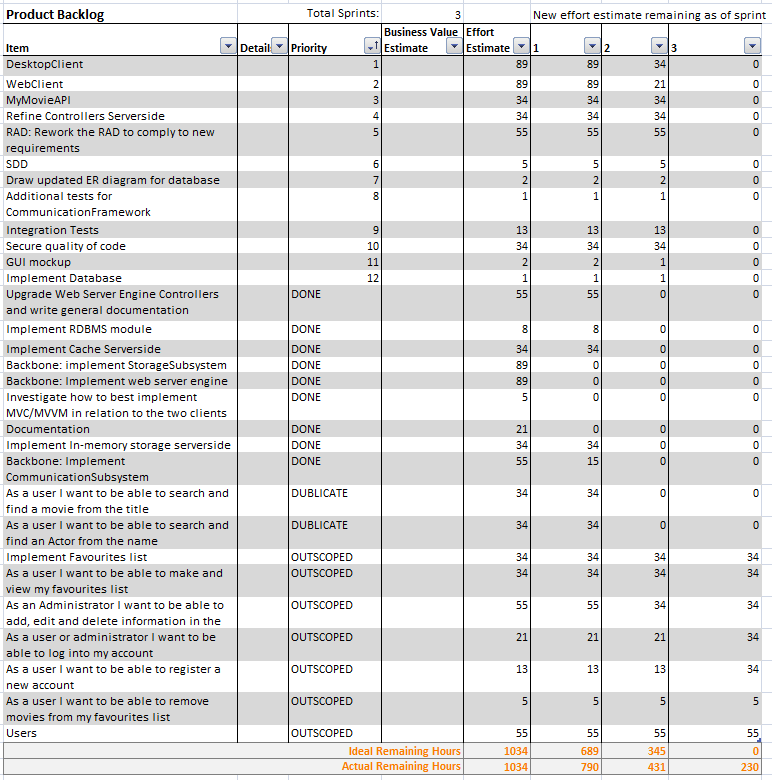
\includegraphics[scale=0.75]{img/SCRUM/productBacklog.PNG}
\caption{Product Backlog}
\label{fig:Product Backlog}
\end{figure}


\subsection{Definition of Done}
\label{sec:Definition of Done}
Definition of done for code:
Done means coded to standards, commented, OCL implemented, unit tested and reviewed by the coders and a second party. Changes affecting documentation or models must be updated accordingly. \\


\noindent Definition of done for documentation:
Documentation is to be done in Latex, with all relevant models included. Sections must have a high quality of writing and be reviewed by a peer. \\
Changes must be documented in the table of change with data and pointing to the relevant section.


\section{Sprint 1}
\label{chap:Spring 1}


\subsection{Backlog}
Below is the backlog for our first sprint
\begin{figure}[h]
\begin{center}
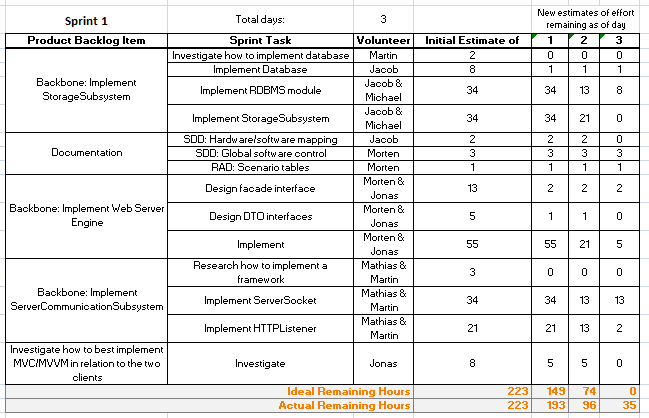
\includegraphics[scale=0.75]{img/SCRUM/backlogSprint1.png}
\caption{Backlog Sprint 1}
\label{fig:Backlog Sprint 1}
\end{center}
\end{figure}

\newpage
\subsection{Burndown}
Below is the burndown for our first Sprint
\begin{figure}[h]
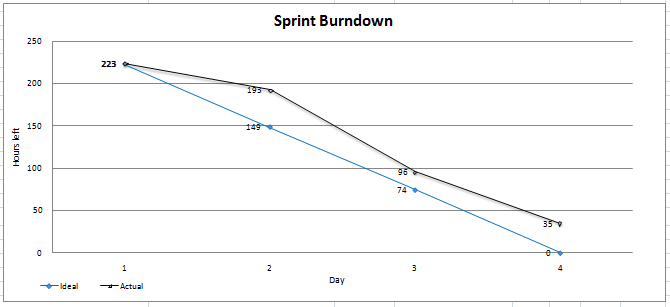
\includegraphics[scale=0.7]{img/SCRUM/burndownSprint1.png}
\caption{Burndown Sprint 1}
\label{fig:Burndown Sprint 1}
\end{figure}


\subsection{Sprint retrospective}

\begin{center}
\begin{tabular}{|c|c|}
\hline \textbf{What's working well} & \textbf{What could work better} \\ 
\hline Mutual interest in different programming tasks & SCRUM \\ 
Pair Responsibilities(XP) & Pair programming (XP) \\ 
 Time Planning &  \\ 
\hline 
\end{tabular} 
\end{center}



\newpage
\section{Sprint 2}
\label{chap:Spring 2}

\subsection{Backlog}
Below is the backlog for our second sprint
\begin{figure}[h]
\begin{center}
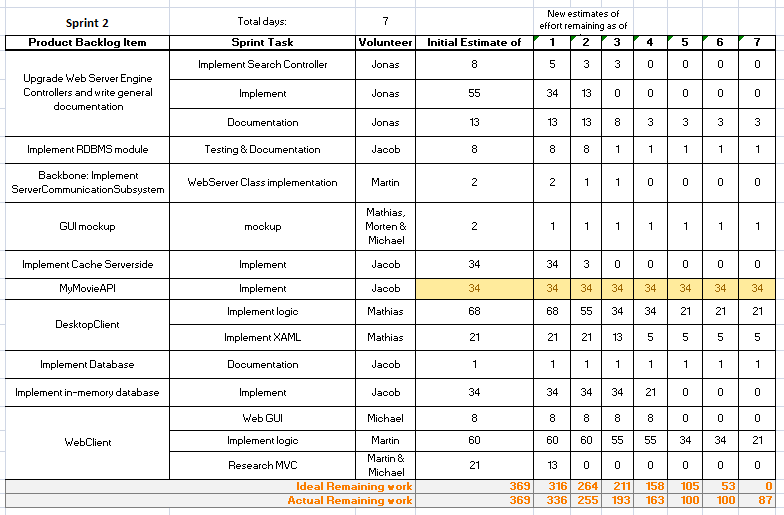
\includegraphics[scale=0.6]{img/SCRUM/backlogSprint2.png}
\caption{Backlog Sprint 2}
\label{fig:Backlog Sprint 2}
\end{center}
\end{figure}

\newpage
\subsection{Burndown}
Below is the burndown for our first Sprint
\begin{figure}[h]
\begin{center}
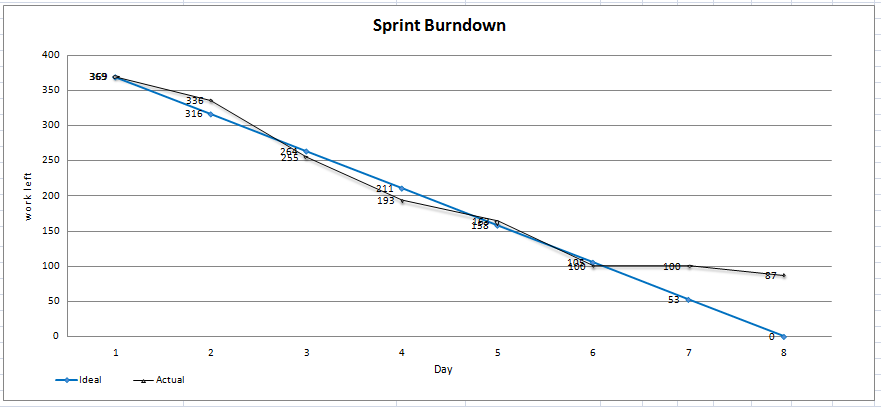
\includegraphics[scale=0.55]{img/SCRUM/burndownSprint2.png}
\caption{Burndown Sprint 2}
\label{fig:Burndown Sprint 2}
\end{center}
\end{figure}


\subsection{Sprint retrospective}

\begin{center}
\begin{tabular}{|c|c|}
\hline \textbf{What's working well} & \textbf{What could work better} \\ 
\hline No pair programming = more Velocity & Big programming tasks have left some in the cold \\ 
\hline 
\end{tabular} 
\end{center}




\newpage
\section{Sprint 3}
\label{chap:Spring 3}
Below is the backlog for our first sprint
\begin{figure}[h]
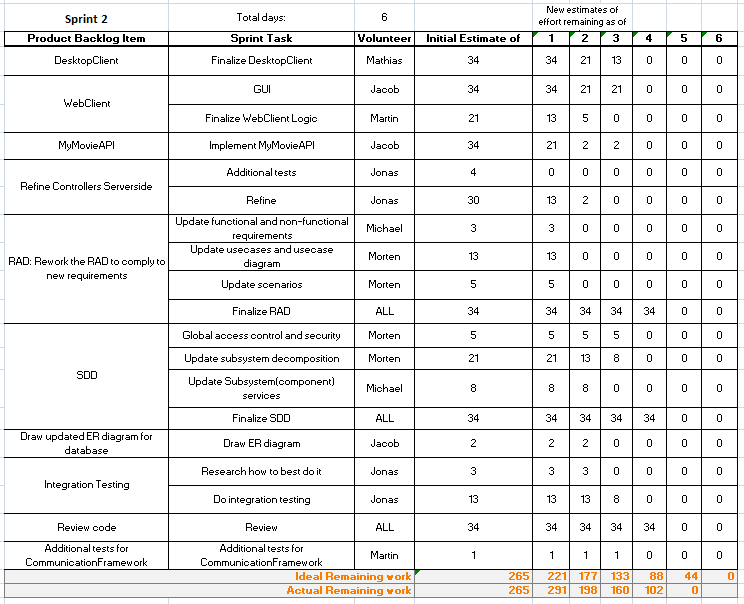
\includegraphics[scale=0.75]{img/SCRUM/backlogSprint3.png}
\caption{Backlog Sprint 3}
\label{fig:Backlog Sprint 3}
\end{figure}

\newpage
\subsection{Burndown}
Below is the burndown for our third and last Sprint
\begin{figure}[h]
\begin{center}
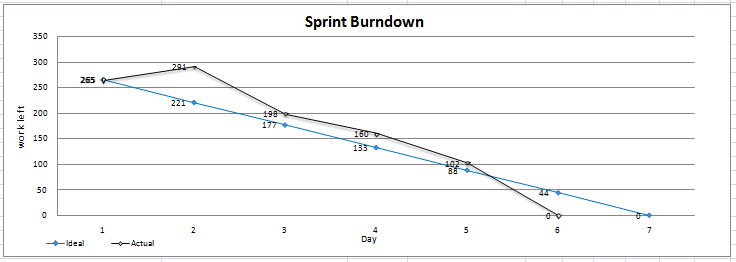
\includegraphics[scale=0.7]{img/SCRUM/burndownSprint3.png}
\caption{Burndown Sprint 3}
\label{fig:Burndown Sprint 3}
\end{center}
\end{figure}



\section{Velocity}
Below is a chart of our velocity


\begin{figure}[h]
\begin{center}
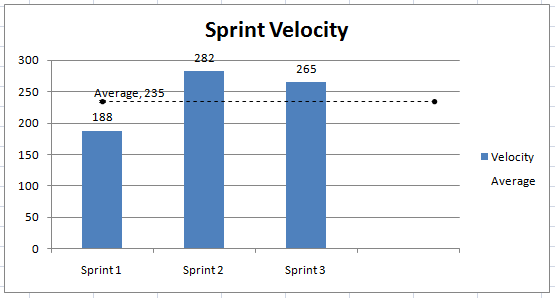
\includegraphics[scale=0.7]{img/SCRUM/overallVelocity.png}
\caption{Velocity}
\label{fig:Velocity}
\end{center}
\end{figure}



\newpage
\section{Release Burndown Chart}
\label{chap:Release Burndown Chart}
\begin{figure}[h]
\begin{center}
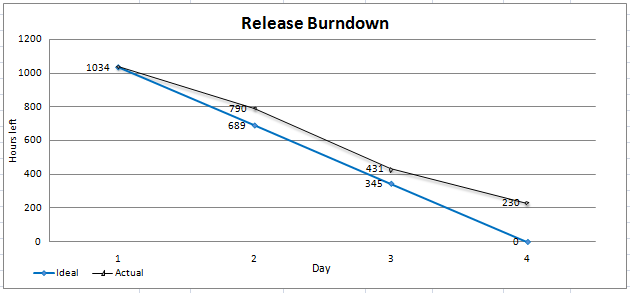
\includegraphics[scale=0.7]{img/SCRUM/releaseBurndown.PNG}
\caption{Release Burndown}
\label{fig:Release Burndown}
\end{center}
\end{figure}





\subsection{Trello}



\begin{figure}[h]
\begin{center}
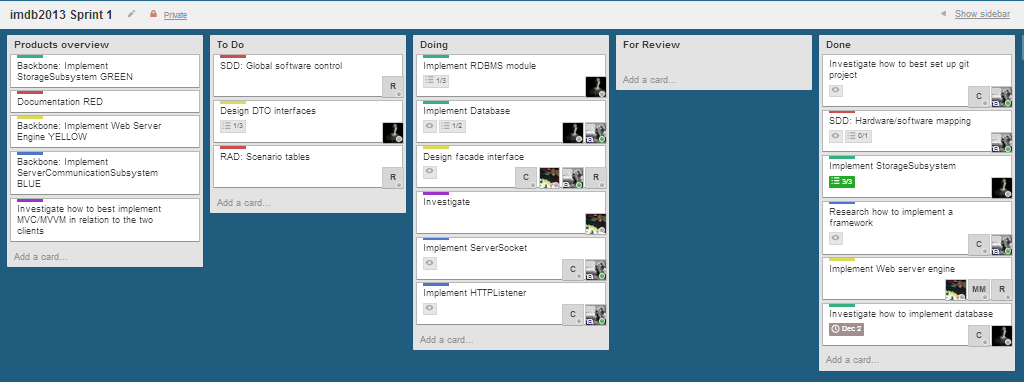
\includegraphics[scale=0.5]{img/SCRUM/trelloSprint1.png}
\caption{Trello Sprint 1}
\label{fig:Trello Sprint 1}
\end{center}
\end{figure}

\begin{figure}[h]
\begin{center}
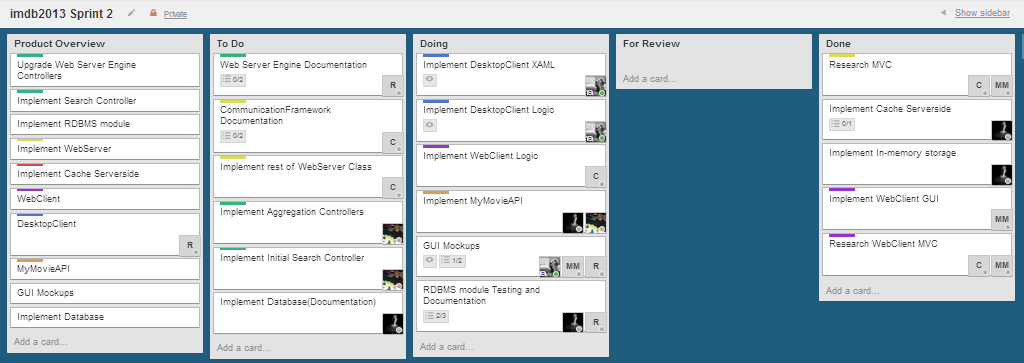
\includegraphics[scale=0.5]{img/SCRUM/trelloSprint2.png}
\caption{Trello Sprint 2}
\label{fig:Trello Sprint 2}
\end{center}
\end{figure}

\begin{figure}[h]
\begin{center}
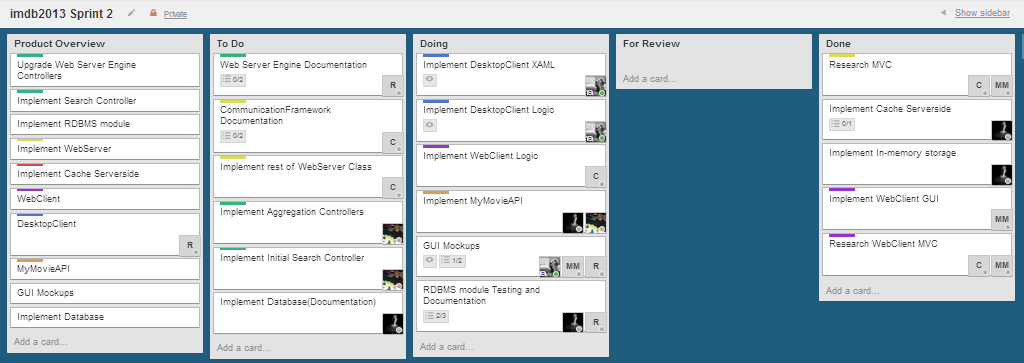
\includegraphics[scale=0.5]{img/SCRUM/trelloSprint2.png}
\caption{Trello Sprint 3}
\label{fig:Trello Sprint 3}
\end{center}
\end{figure}          
